\documentclass[10pt]{standalone}
\usepackage{pgfplots}
\pgfplotsset{compat=1.15}
\usepackage{mathrsfs}
\usetikzlibrary{arrows}
\pagestyle{empty}
\begin{document}
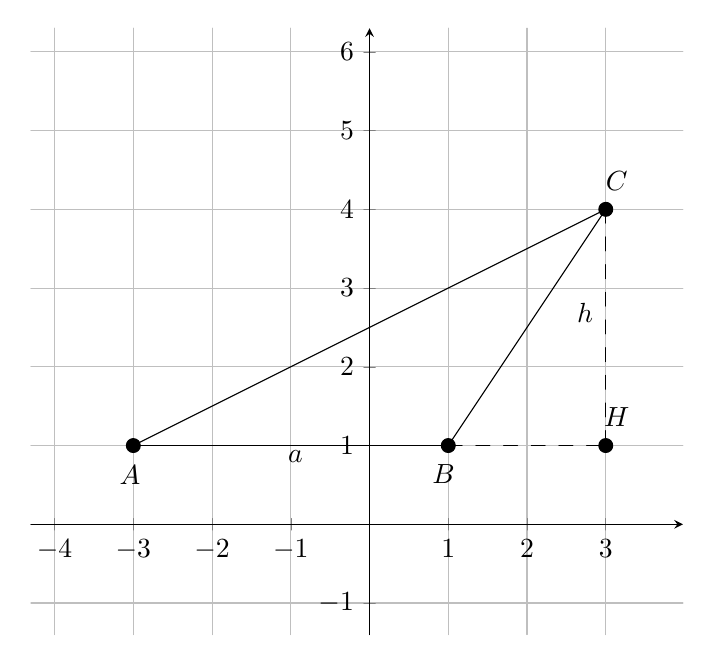
\begin{tikzpicture}[line cap=round,line join=round,>=triangle 45,x=1.0cm,y=1.0cm]
\begin{axis}[
x=1.0cm,y=1.0cm,
axis lines=middle,
ymajorgrids=true,
xmajorgrids=true,
xmin=-4.3,
xmax=3.9799999999999978,
ymin=-1.4,
ymax=6.299999999999998,
xtick={-4.0,-3.0,...,3.0},
ytick={-1.0,0.0,...,6.0},]
\clip(-4.3,-1.4) rectangle (3.98,6.3);
\draw  (-3.,1.)-- (1.,1.);
\draw  (1.,1.)-- (3.,4.);
\draw  (3.,4.)-- (-3.,1.);
\draw [dash pattern=on 5pt off 5pt] (1.,1.)-- (3.,1.);
\draw [dash pattern=on 5pt off 5pt] (3.,4.)-- (3.,1.);
\begin{scriptsize}
\draw [fill=black] (-3.,1.) circle (2.5pt);
\draw[color=black] (-3.0414,0.6206) node {$A$};
\draw [fill=black] (1.,1.) circle (2.5pt);
\draw[color=black] (0.9386,0.6406) node {$B$};
\draw [fill=black] (3.,4.) circle (2.5pt);
\draw[color=black] (3.1386,4.3606) node {$C$};
\draw[color=black] (-0.9414,0.8606) node {$a$};
\draw [fill=black] (3.,1.) circle (2.5pt);
\draw[color=black] (3.1386,1.3606) node {$H$};
\draw[color=black] (2.7386,2.6806) node {$h$};
\end{scriptsize}
\end{axis}
\end{tikzpicture}
\end{document}